\documentclass[14 pt]{extarticle}
\usepackage[utf8]{inputenc} 
\usepackage[T1,T2A]{fontenc}
\usepackage[english, ukrainian]{babel}
\usepackage[center]{titlesec}
\usepackage{amsmath, amsfonts}
\usepackage{mathtools}
\usepackage{marvosym}
\usepackage{geometry}
\geometry{verbose,a4paper,tmargin=1.5cm,bmargin=1.5cm,lmargin=1.2cm,rmargin=2cm}
\usepackage{diagbox}
\usepackage{hyperref}
\usepackage{nicefrac}
\usepackage{graphicx}
\usepackage{pgfplots}
\usepackage{physics}
\usepackage{relsize}
\usepackage{textgreek}
\usepackage{upgreek}
\usepackage{adjustbox}
\usepackage{pdfpages}
\linespread{1.3}
\makeatletter
\renewcommand*\env@matrix[1][\arraystretch]{%
  \edef\arraystretch{#1}%
  \hskip -\arraycolsep
  \let\@ifnextchar\new@ifnextchar
  \array{*\c@MaxMatrixCols c}}
\makeatother

\usepgfplotslibrary{fillbetween}
\usepackage{float}
\hypersetup{
    colorlinks=true,
    linkcolor = blue,
}
\DeclareMathOperator*{\argmax}{argmax} % thin space, limits underneath in displays
\usepackage{tikz}
\newcommand*\circled[1]{\tikz[baseline=(char.base)]{
            \node[shape=circle,draw,inner sep=2pt] (char) {#1};}}

            


\begin{document}



\begin{titlepage}
    \begin{center}
        
        
\includegraphics[width=18cm]{image1.png}
        Мiнiстерство освiти i науки України \\
        Національний технічний університет України \\
        «Київський політехнічний інститут імені Ігоря Сікорського» Iнститут прикладного системного аналiзу \\

        \vspace{4.5cm}
        \textbf{Лабораторна робота № 4}\\
        з курсу «Чисельнi методи» \\
        з теми «Наближення функцій» \\
        Варіант № 9 \\
    \end{center}

    \vspace{2cm}

    \begin{flushright}
        Виконав студент 2 курсу групи КА-02 \\
        Романович Володимир Володимирович \\
        перевiрила старший викладач \\
        Хоменко Ольга Володимирiвна \\

    \end{flushright}

    \vfill
    \begin{center}
        Київ -- 2022
    \end{center}
\end{titlepage}
\begin{center}
    \Large
    Задача 1
\end{center}
$$
    y = x^2+6x+8-2e^{x+2}
$$
Виберемо відрізок інтерполяції [-6;0], та виберемо 4 вузли, відстань між якими буде однаковою $x_1 = -6, x_2 = -4, x_3 = -2, x_4 = 0$
\\Значення функції в цих точках: \\ 
\begin{tabular}{|c|c|c|c|c|} \hline
    x& $-6$ & $-4$ & $-2$ & 0 \\ \hline 
    y& $7.963369$&$-0.2706706$&$-2$&$-6.778112$ \\ \hline
\end{tabular} \\ \\ 
Побудуємо таблицю скінченних різниць(обчислено в .ipynb файлі): \\ 
\begin{tabular}{|c|c|c|c|c|} \hline 
    $x_i$ & $y_i$ & $\Delta y_i$ & $\Delta^2 y_i$ & $\Delta^3 y_i$ \\ \hline 
    $-6$ & 7.96 & $-8.23404$ & 6.50471 & $-9.55349$ \\ \hline    
    $-4$ & $-0.27$ & $-1.72933$ & $-3.04878$ &  \\ \hline   
    $-2$ & $-2$ & $-4.77811$ & & \\ \hline
    0 & $-6.78$ & & & \\ \hline
\end{tabular} \\ \\ 
Знайдемо поліном Лагранжа:
\begin{align*}
    L_3(x) = \sum_{i=0}^3 y_i \prod_{j=0,j \neq i}^3 \frac{x-x_j}{x_i-x_j} = 
    y_0 \cdot \frac{(x-x_1 )(x-x_2 )(x-x_3 )}{(x_0 - x_1 )(x_0 - x_2 )(x_0 - x_3 )} +\\  
    y_1 \cdot \frac{(x-x_0 )(x-x_2 )(x-x_3 )}{(x_1 - x_0 )(x_1 - x_2 )(x_1 - x_3 )} +
    y_2 \cdot \frac{(x-x_0 )(x-x_1 )(x-x_3 )}{(x_2 - x_0 )(x_2 - x_1 )(x_2 - x_3 )} +\\
    y_3 \cdot \frac{(x-x_0 )(x-x_1 )(x-x_2 )}{(x_3 - x_0 )(x_3 - x_1 )(x_3 - x_2 )} 
\end{align*}
$$
L_3(x) \approx 
7.9634 \cdot \frac{(x+4)(x+2)x}{-2 \cdot (-4) \cdot (-6)} 
-0.2707 \cdot \frac{(x+6)(x+2)x}{2 \cdot (-2) \cdot (-4)}
- 2 \cdot \frac{(x+6)(x+4)x}{4 \cdot 2 \cdot (-2)} - $$$$
-6.7781 \cdot \frac{(x+6)(x+4)(x+2)}{6 \cdot 4 \cdot 2} = 
\frac{-11942x^3 - 94518x^2 - 284611x - 406686}{60000} \approx 
$$
$$
\approx -(0.199x^3 + 1.575 x^2 + 4.744 x + 6.778)
$$
Перший і другий поліноми Ньютона реалізовані програмно на Python. \\ 
Знайдемо значення поліномів Лагранжа та Ньютона в деяких невузлових точках \\  $\tilde{x}_1 = -5, \tilde{x}_2 = -3, \tilde{x}_3 = -1, \tilde{x}_4 = -2.1$, та порівняємо із значенням заданої функції в цих точках \\ 
\begin{tabular}{|c|c|c|c|c|} \hline
    $\tilde{x}_i$&$f(x)$ & $Lagrange$ & $Newton 1$ & $Newton 2$ \\ \hline    
    $-5$&2.90042586 & 2.43616706&2.43616706&2.43616706 \\ \hline
    $-3$&$-1.73575888$& $-1.35133073$&$-1.35133073$&$-1.35133073$ \\ \hline
    $-1$&$-2.43656366$&$-3.41086496$&$-3.41086496$&$-3.41086496$ \\ \hline
    $-2.1$&$-1.99967484$&$-1.92053835$&$-1.92053835$&$-1.92053835$ \\ \hline
\end{tabular} \\ 
Побудуємо інтерполяційний кубічний сплайн за таблицею:
\begin{tabular}{c|c|c|c|}
    x&$-4$&$-2$&$0$ \\ \hline
    y&$-0.271$&$-2$&$-6.778$
\end{tabular}:
$$
g(x) = \begin{cases}
    g_1, x \in [-4;-2] \\ 
    g_2, x \in [-2;0]
\end{cases}
=\begin{cases}
    a_1 + b_1 (x+2) + c_1 (x+2)^2 + d_1 (x+2)^3, & x \in [-4;-2] \\ 
    a_2 + b_2 x + c_2 x^2 + d_2 x^3, & x \in [-2;0]
\end{cases}
$$
$$
\begin{cases}
    a_1 + b_1 (-4+2) + c_1 (-4+2)^2 + d_1 (-4+2)^3 = -0.271 \\ 
    a_2 - 2 b_2 + 4 c_2 - 8 d_2 = -2 \\ 
    a_2 + 0 \cdot b_2 + 0 \cdot c_2 + 0 \cdot d_2 = -6.778
\end{cases} \implies$$$$ \implies
\begin{cases}
    a_1 - 2b_1 + 4 c_1 - 8 d_1 = -0.271 \\ 
    a_2 - 2 b_2 + 4 c_2 - 8 d_2 = -2 \\ 
    a_2 = -6.778
\end{cases}
$$
З неперервності сплайну: $g_1(-2) = g_2(-2), g_1'(-2) = g_2'(-2), g_1''(-2) = g_2''(-2)$
\\ 
$g_1'(x) = b_1 + 2c_1 (x+2) + 3d_1 (x+2)^2,\\ g_2'(x) = b_2 + 2c_2 x + 3d_2 x^2$ \\ 
$g_1''(x) = 2c_1 + 6d_1 (x+2)$ \\ 
$g_2''(x) = 2c_2 + 6d_2 x$ \\
Також умовою сплайну є $g_1''(-4)=0, g_2''(0)=0$\\ 
Отже маємо таку систему:
$$
\begin{cases}
    a_1 - 2b_1 + 4 c_1 - 8 d_1 = -0.271 \\ 
    a_2 - 2 b_2 + 4 c_2 - 8 d_2 = -2 \\ 
    a_2 = -6.778 \\ 
    a_1 = a_2 -2 b_2 + 4 c_2 - 8 d_2 \\
    b_1 = b_2 - 4 c_2 +12 d_2 \\ 
    2c_1 = 2c_2 - 12d_2 \\ 
    2c_1 - 12 d_1 = 0 \\ 
    2c_2 = 0
\end{cases} \implies
\begin{cases}
    a_1 = 2b_1 - 4 c_1 + 8 d_1 - 0.71 \\ 
    a_1 = a_2 - 2 b_2 + 4 c_2 - 8d_2 \\ 
    a_2 - 2 b_2 + 4 c_2 - 8 d_2 = -2 \\
    a_2 = -6.778 \\ 
    b_1 = b_2 - 4c_2 + 12d_2 \\ 
    c_1 = c_2 - 6d_2 \\ 
    c_1 = 6d_1 \\ 
    c_2 = 0 
\end{cases} \implies
$$
$$\implies
\begin{cases}
    a_1 = -2 \\
    a_2 = -6.778 \\ 
    - 2b_1+16 d_1 = 1.729 \\ 
    b_2= -(2.389 + 4 d_2) \\ 
    b_1 = -2.389 -8 d_1 \\ 
    d_1 = -d_2 \\ 
    c_1 = 6 d_1 \\ 
    c_2 = 0
\end{cases} \implies
\begin{cases}
    a_1 = -2 \\ 
    a_2 = -6.778 \\ 
    b_1 = -1.62675\\
    b_2 = -2.770125 \\ 
    c_1 = -0.5716875 \\ 
    c_2 = 0 \\ 
    d_1 = -0.09528125 \\ 
    d_2 = 0.09528125 
\end{cases} \implies
$$
$$
g(x)
=\begin{cases}
    -2 - 1.62675 (x+2) -0.5716875 (x+2)^2 -0.09528125 (x+2)^3, & x \in [-4;-2] \\ 
    -6.778 -2.770125 x + 0.09528125 x^3, & x \in [-2;0]
\end{cases}
$$
Зобразимо графіки всіх знайдених інтерполяцій \\ 
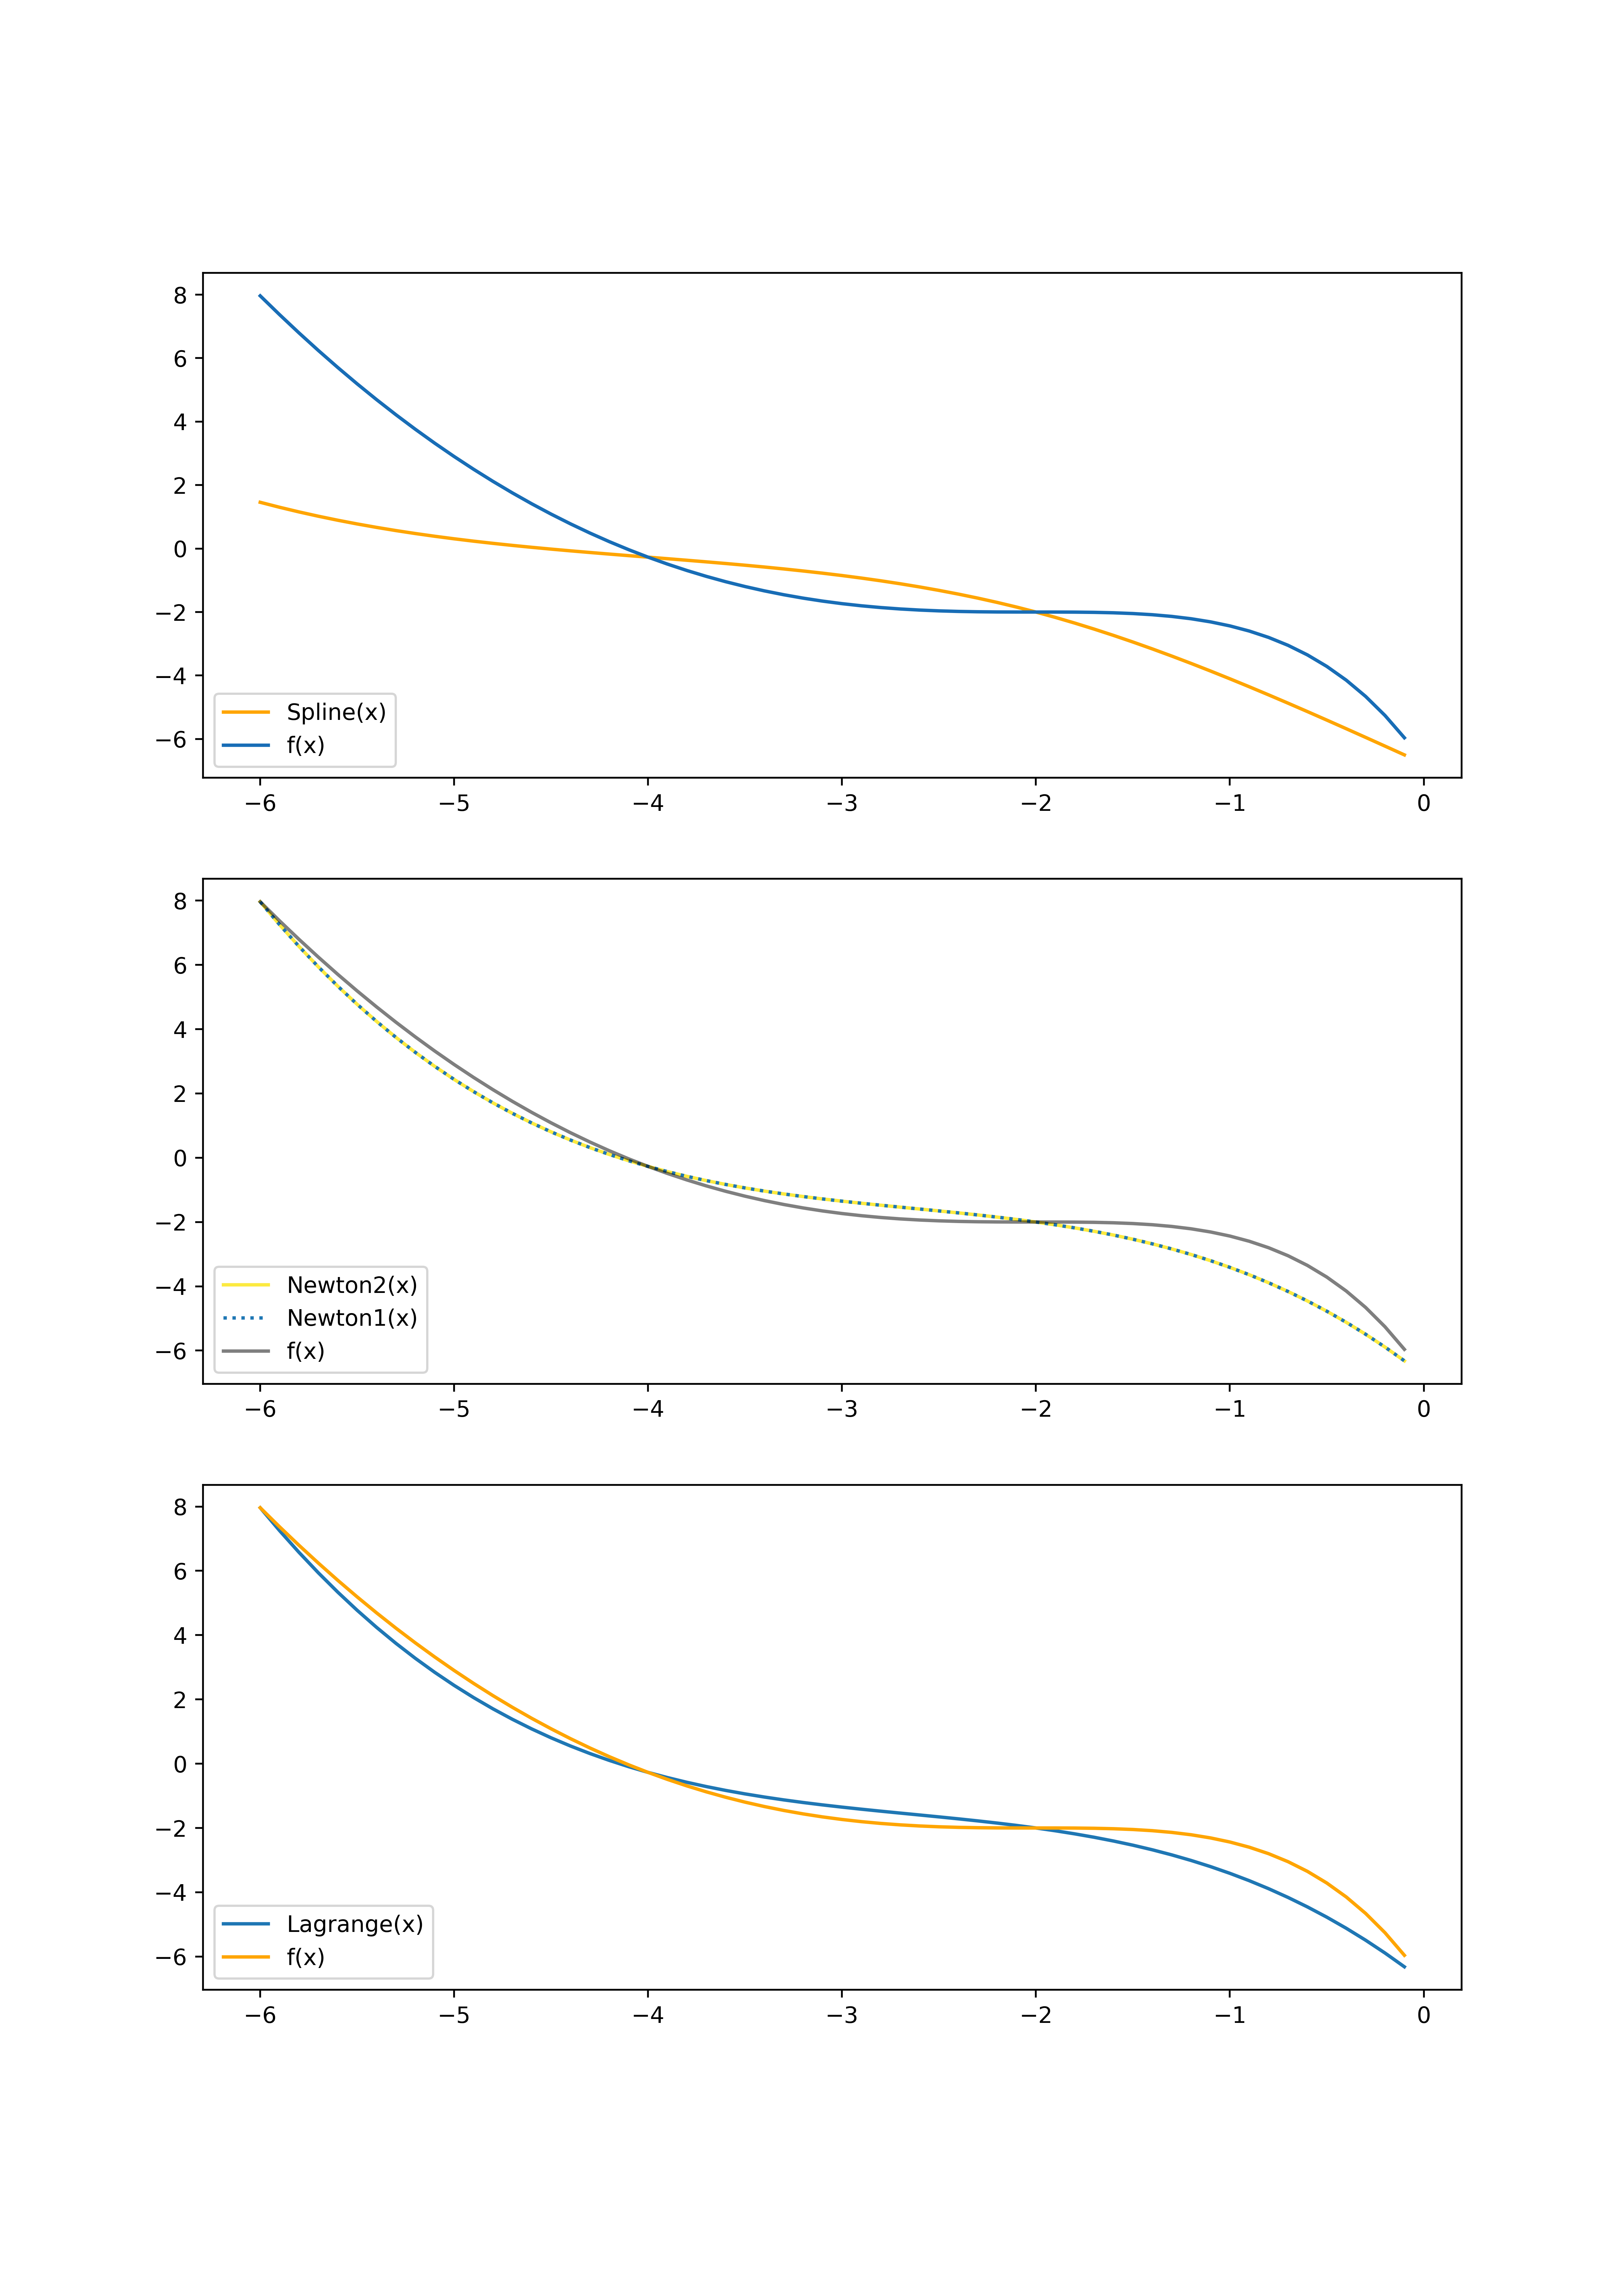
\includegraphics[width = 11.8cm]{plots.png}
\begin{center}
    \Large
    Задача 2
\end{center}
\begin{tabular}{|c|c|c|c|c|c|c|c|c|c|c|c|} \hline
    x &2&2.22&2.44&2.67&2.89&3.11&3.33&3.56&3.78&4 \\ \hline
    y &1.52&1.84&1.68&1.34&1.67&1.35&1.44&1.43&0.91&1.09 \\ \hline
\end{tabular}\\ \\
Зобразимо точки на графіку: \\ 
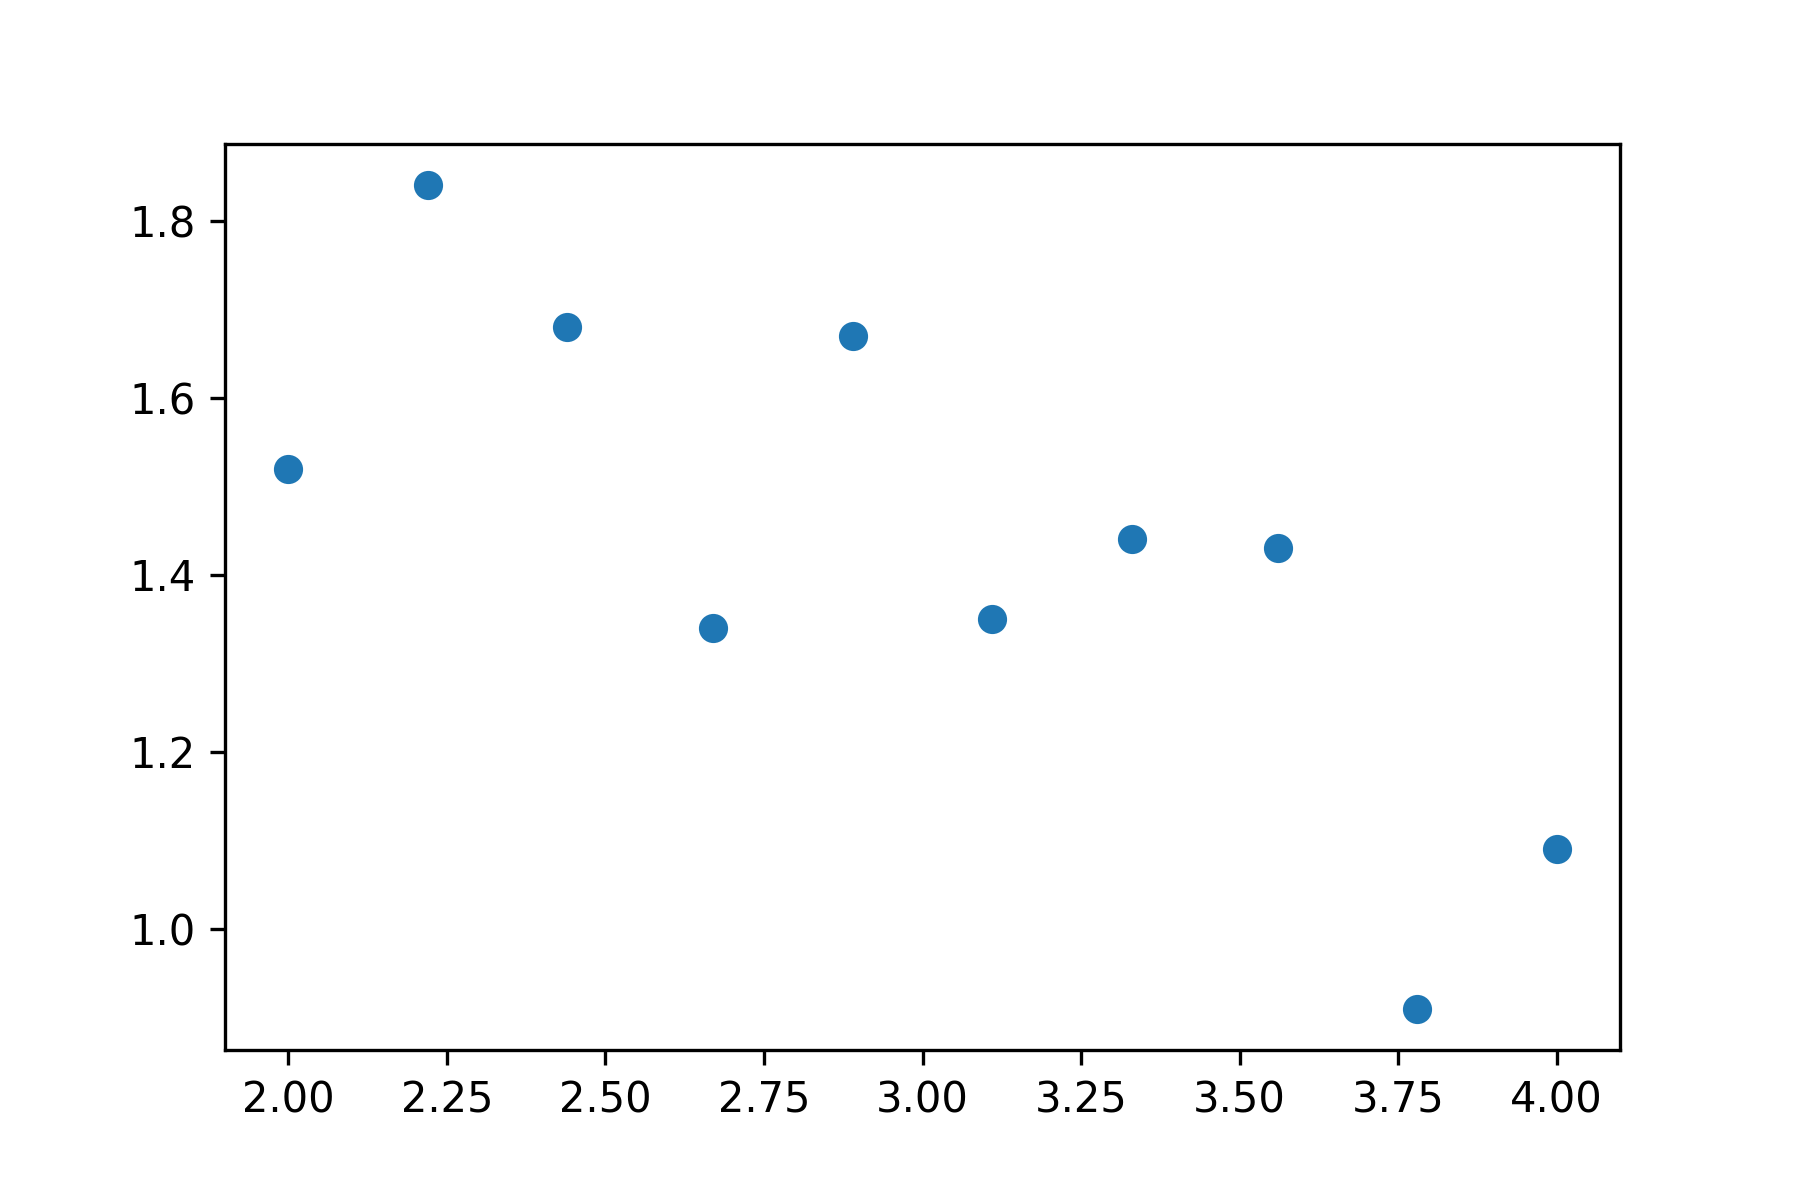
\includegraphics[width=10cm]{scatter.png} \\ 
Бачимо що розташування точок нагадує параболу вітками вниз. Тому як апроксимуючу фукнцію виберемо $y = c + bx + ax^2$ \\ 
Запрограмувавши метод найменших квадратів отримали \\ 
$y = 0.8294147 +  0.76511646x -0.18044811x^2$ \\ 
Наведемо графік цієї функції разом з заданими точками: \\ 
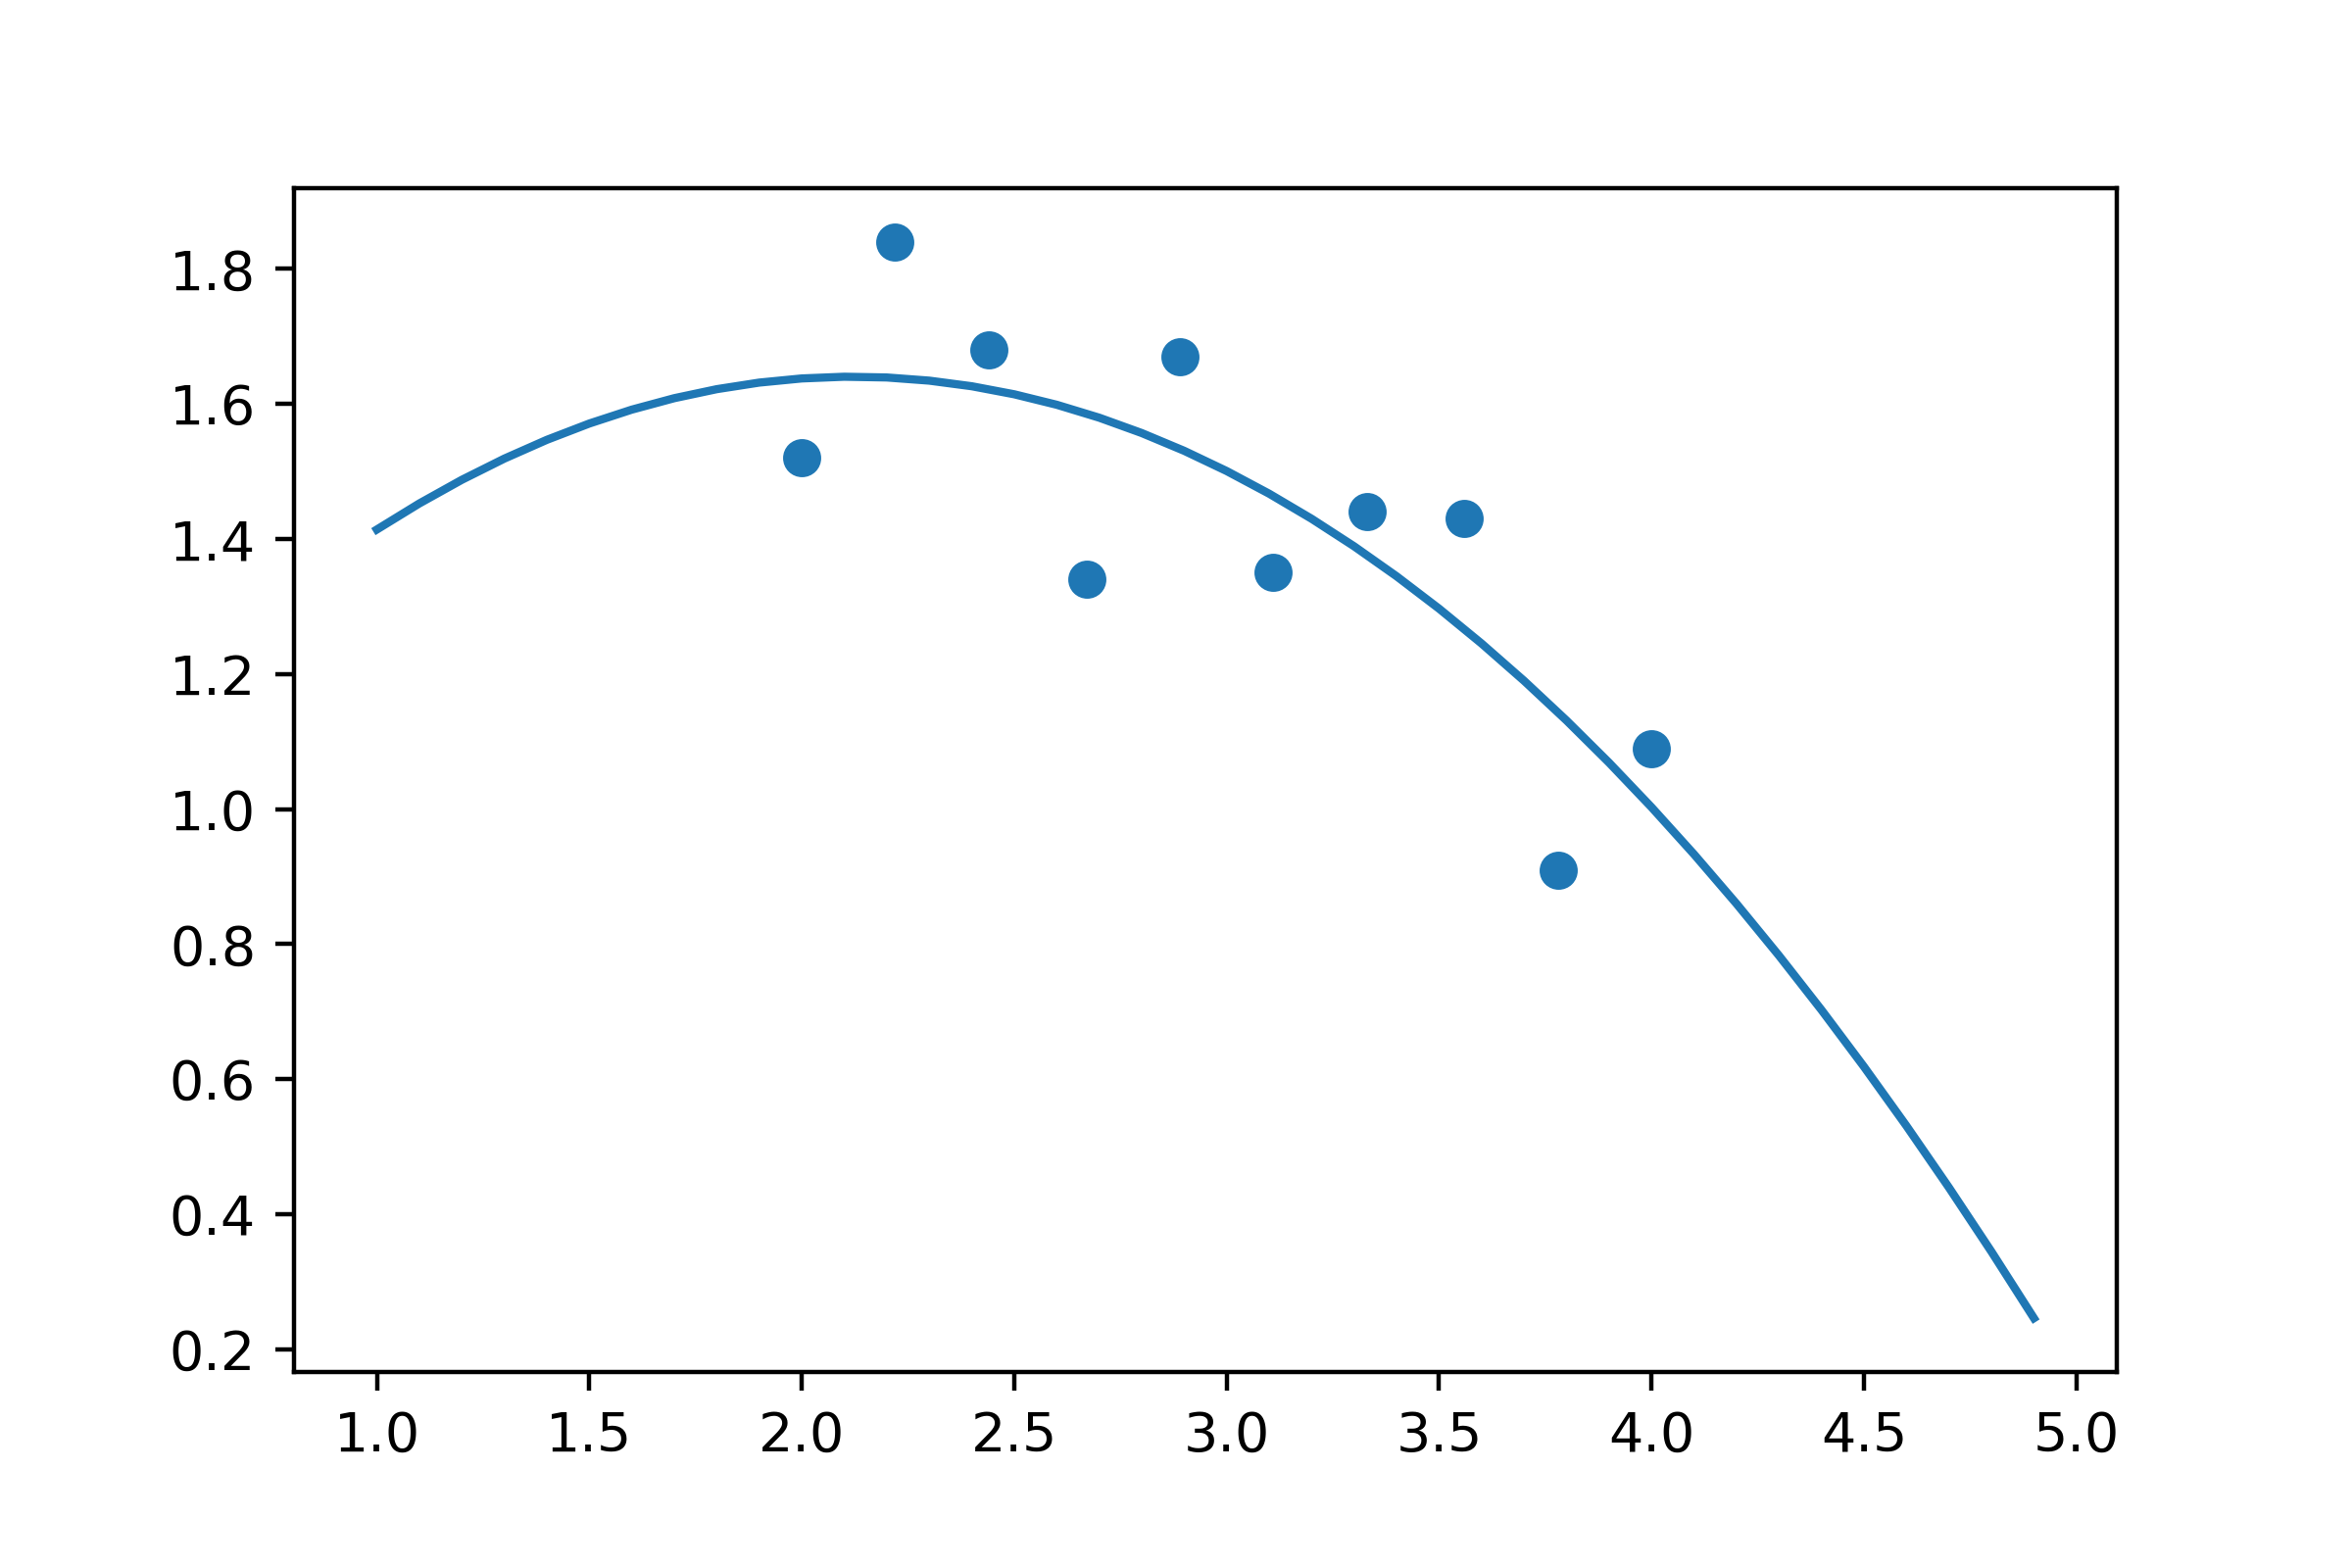
\includegraphics{plot2.png}
\newpage
\begin{center}
    \Large
    Висновки
\end{center}
\textbf{В першому завданні} вибравши 4 вузла нашої функції ми
 побудували поліноми Лагранжа та Ньютона на відрізку [-6;0], а також кубічний сплайн дефекту 1.\\
Видно що поліноми Лагранжа та Ньютона краще наблизили функцію. Проте порівнявши деякі невузлові
точки поліномів та заданої функції отримали достатьно великі розбіжності. Це зв'язано з тим,
що ми будували інтерполяцію а не апроксимацію, тому, як ми можемо побачити в точки х=-2.1, яка близька 
до вузла, різниця між заданою функцією та значеннями поліномів є невеликою, а із збільшенням 
відстані від вузлів, наближення стає все менш точним. \\ 
\textbf{В другому завданні} ми зобразили задані точки на координатній площині, і з їх
розташування вибрали апроксимуючу функцію -- параболу. Обчисливши коефіціенти за методом
найменших квадратів отримали таку функцію $y = 0.8294147 +  0.76511646x -0.18044811x^2$. 
Побудувавши її графік переконались, що дійсно, крива непогано апроксимує функцію, точки якої нам задані. 
\\ 
\textbf{Лістинг програми:}



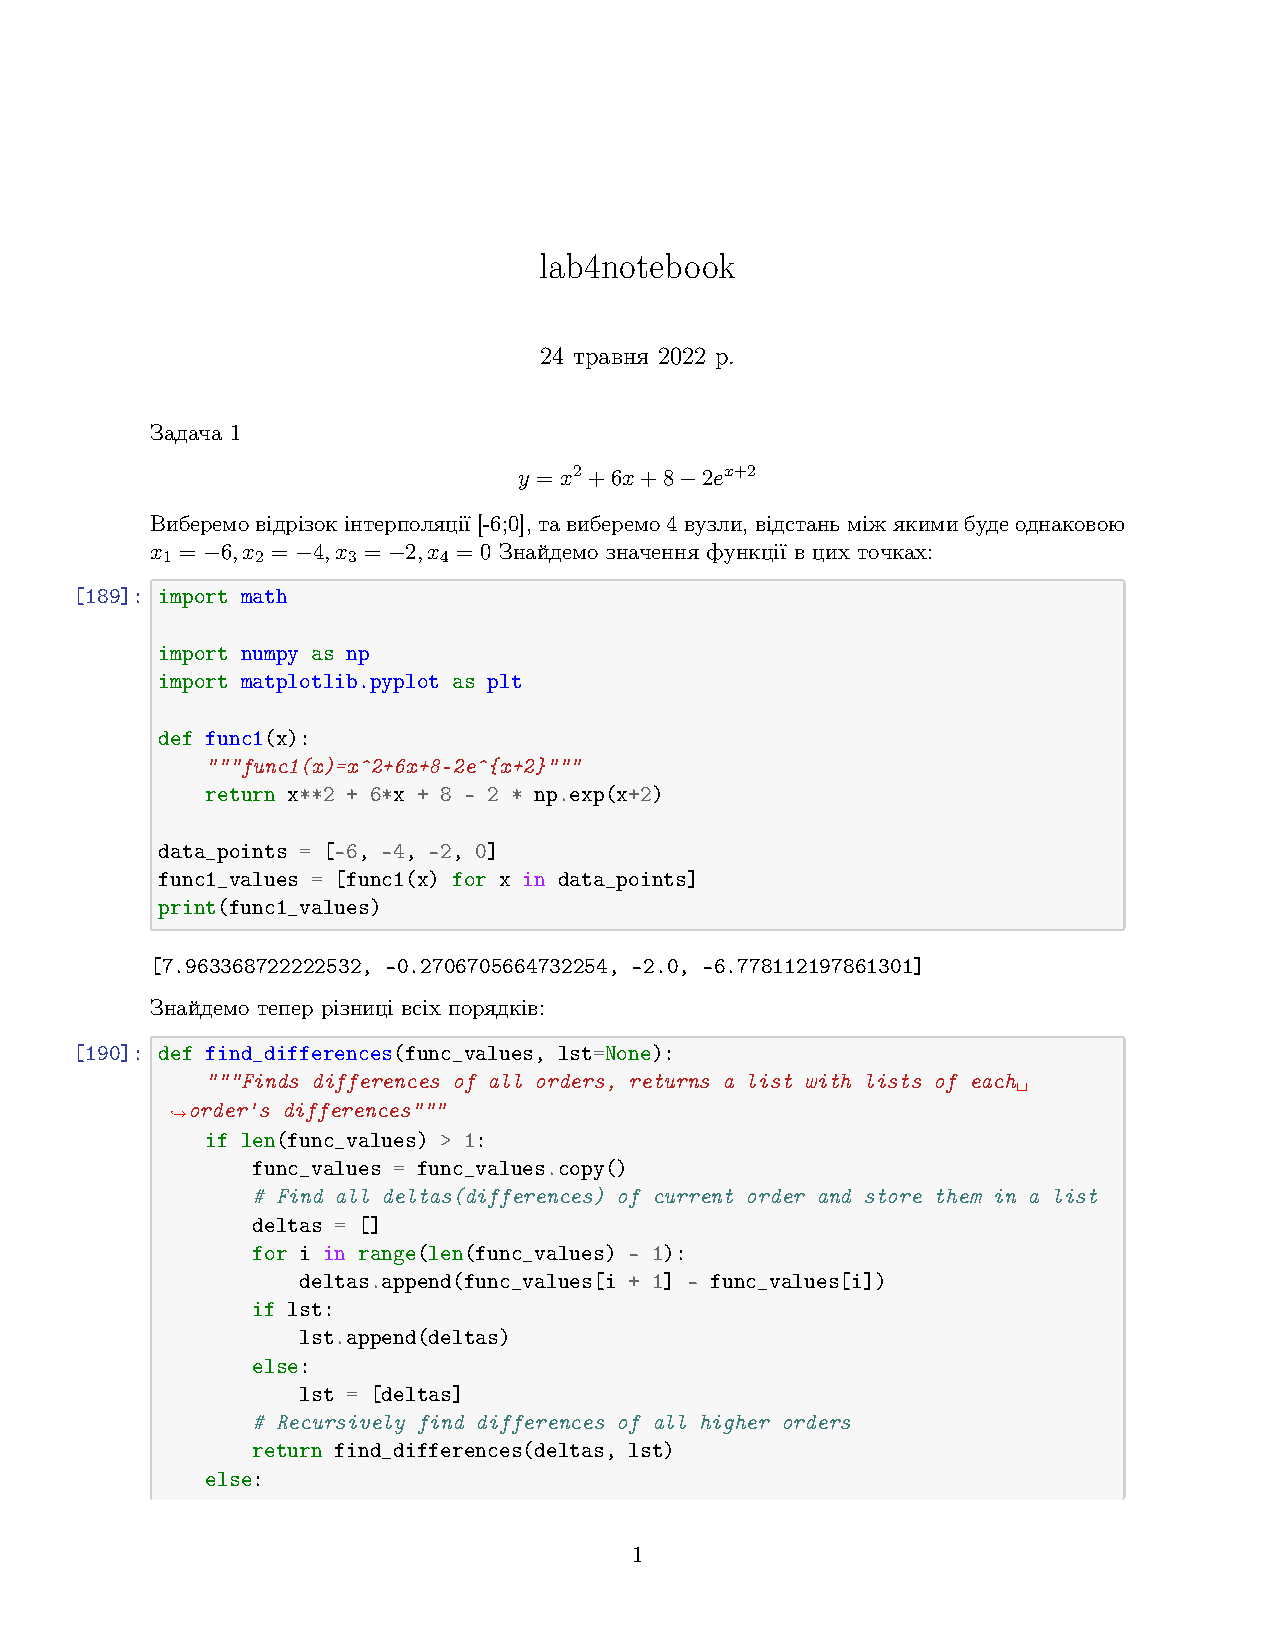
\includepdf[pages=-]{lab4notebook.pdf}

\end{document}


